%E for even page O for odd page L for left side C for centered R for right side
\pagestyle{fancy}
\fancyhf{}
\fancyhead[R]{\textcolor{gray}{\scriptsize Last update \today}}
% \fancyhead[RE,LO]{Guides and tutorials}
% \fancyfoot[CE,CO]{\leftmark}
\fancyfoot[C]{\thepage}

% \pagecolor{gray!20}\afterpage{\nopagecolor}
% \colorbox{gray!20!white}{
\begin{minipage}{0.32\columnwidth}

    \tikz[remember picture,overlay]
    \draw [fill, gray!20!white] (current
    page.north west) rectangle +(0.39\paperwidth,-1.0\paperheight);

    \vspace*{-16.5mm}
    \noindent
    {\color{black!75!white}\rule{1.06\linewidth}{0.15mm} }

    \vspace*{-10mm}
    \begin{flushright}
        \textcolor{my_blue}{\bf\Large Telephone}\\ \vspace*{3mm}

        (64) 204 1437112 \\ \vspace*{-0.5mm}
        (64) 9 414 0800 ext. 43599\\
        \vspace*{4mm}

        \textcolor{my_blue}{\bf\Large Zoom/Skype}\\ \vspace*{3mm}

        edisonffh%@outlook.com\\
        \vspace*{4mm}

        \textcolor{my_blue}{\bf\Large eMail}\\ \vspace*{3mm}

        \href{mailto:edisonffh@gmail.com}{\textbf{edisonffh@}\\[-1mm]gmail.com}\\

        \href{mailto:e.florez@massey.ac.nz}{\textbf{e.florez@}\\[-2mm]massey.ac.nz}\\
        \vspace*{6mm}

        \textcolor{my_blue}{\bf\Large Key Skills}\\
        %\vspace*{3mm}
        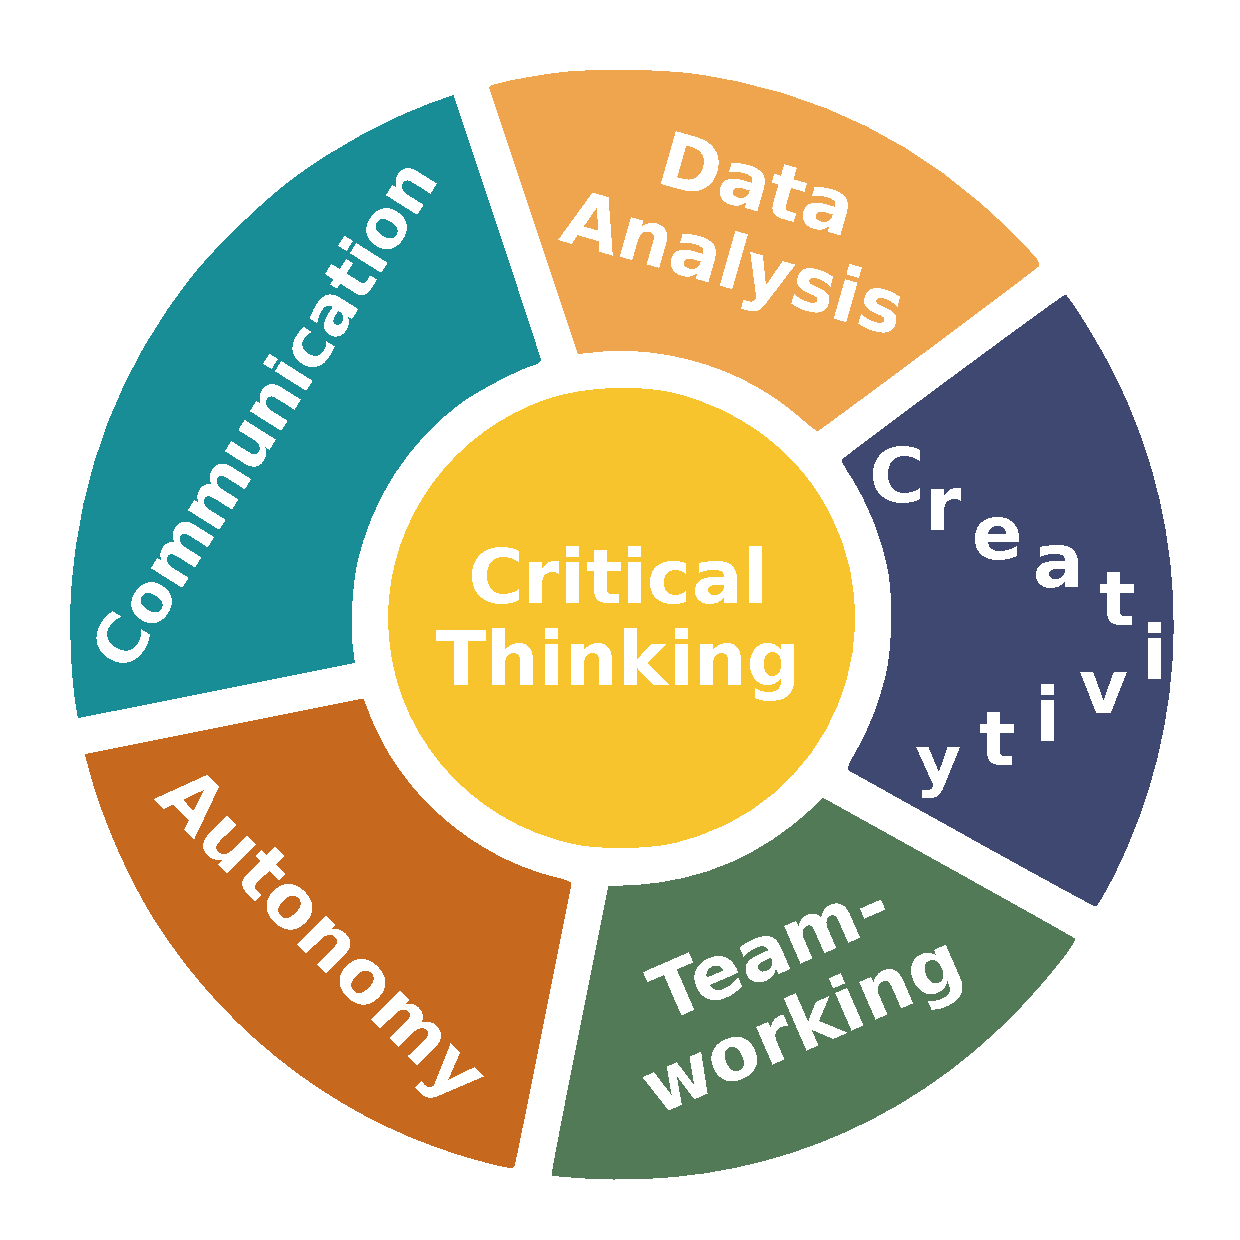
\includegraphics[scale=0.3]{figs/skills1.pdf}\\
        \vspace*{4mm}

        \textcolor{my_blue}{\bf\Large Technical Skills}\\ \vspace*{4mm}

        \textcolor{my_blue}{\bf\large \textbullet~~ OS Preference}\\
        \vspace*{3mm}

        %     {GNU/Linux }
\includegraphics[scale=0.25]{figs/5stars.pdf}
        {GNU/Linux
        }
\includegraphics[width=1.5cm,height=0.27cm]{figs/5stars.pdf}\\
        %\vspace*{-1mm}
        {Windows
        }
\includegraphics[width=1.5cm,height=0.22cm]{figs/4-8stars.pdf}\\
        %\vspace*{-1mm}
        {MacOS
        }
\includegraphics[width=1.5cm,height=0.19cm]{figs/4stars.pdf}\\
        \vspace*{4mm}

        \textcolor{my_blue}{\bf\large \textbullet~~ Programming}\\
        %\vspace*{3mm}
        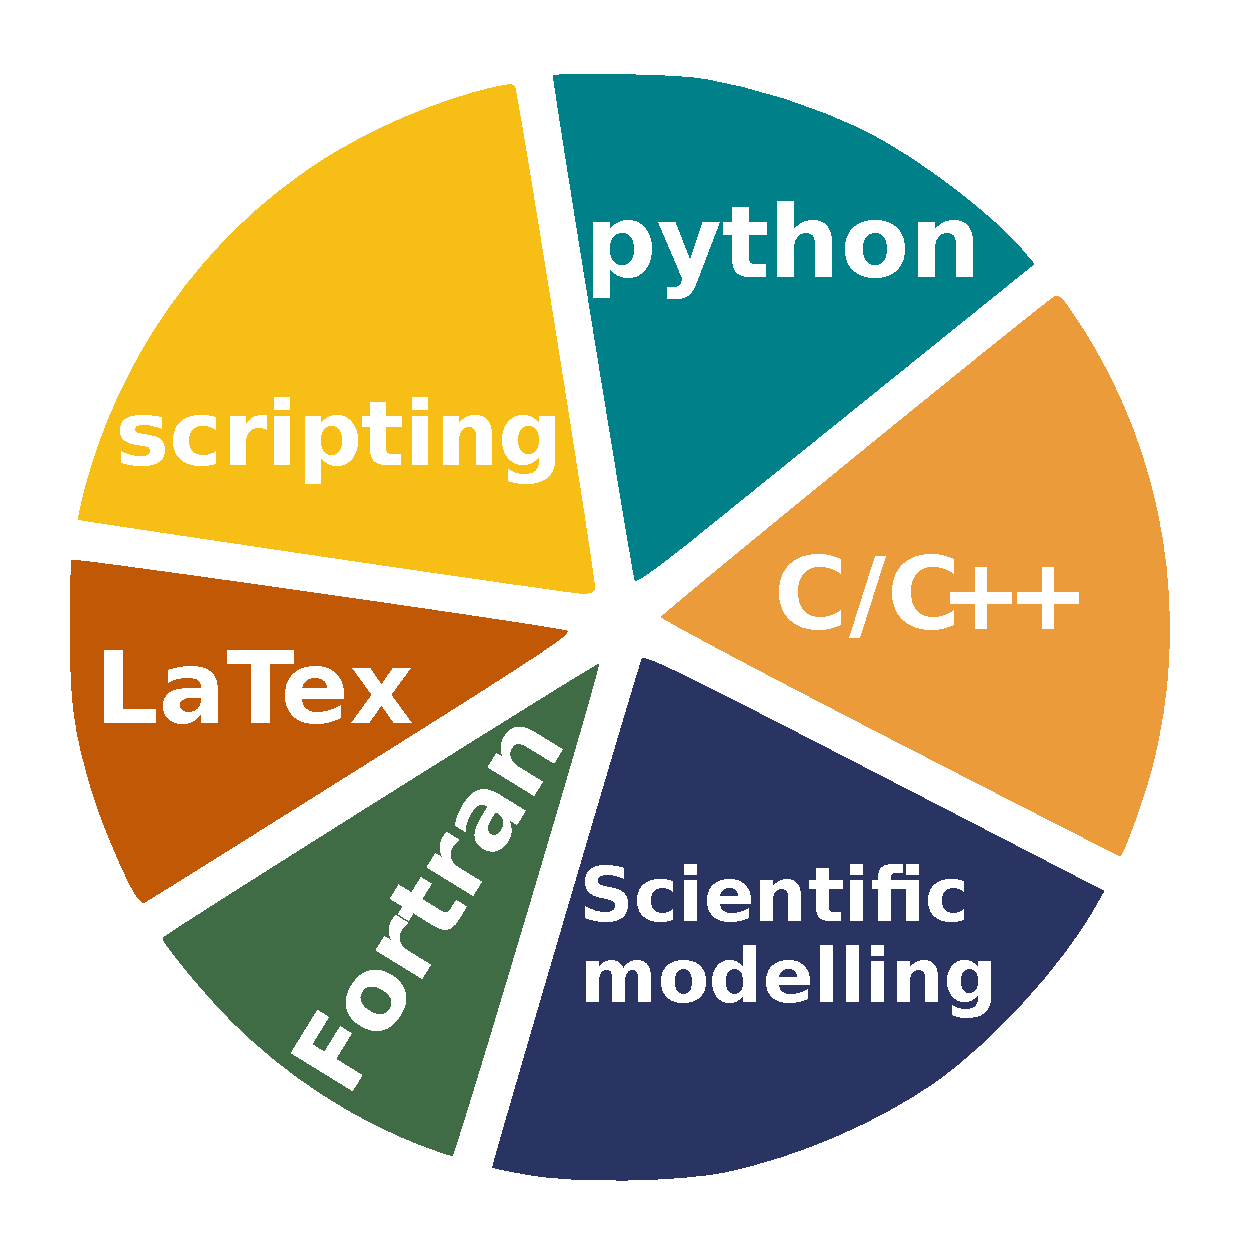
\includegraphics[scale=0.3]{figs/programming1.pdf}\\
        %      \vspace*{5mm}

    \end{flushright}
\end{minipage}
% }
\begin{minipage}{0.1\columnwidth}
\end{minipage}
\begin{minipage}{0.1\columnwidth}
\end{minipage}
\begin{minipage}{0.1\columnwidth}
\end{minipage}
%----------------------------------------------------
\begin{minipage}{0.62\columnwidth}

\vspace*{-5mm}
\begin{flushright}
    {{\fontsize{40}{60}\selectfont Edison\bf Florez}\\[5pt]
        \textcolor{my_blue}{\bf\Large Computational Chemist}}
\end{flushright}

\vspace*{-1mm}
\hspace*{-1.9mm}
\noindent
{\color{gray!20!white} \rule{1.01\linewidth}{3mm} }

%----------------------------------------------------

\vspace*{-5mm}
{\bf\large Profile:}
I want to understand chemistry at its most fundamental level by using  computers. Quantum Chemistry is used in a variety of ways to analyze and explain interesting problems of science. In what I do, not only do you learn about chemistry, biology or physics, but you also learn how to use a computer and how to write programs to build models and simulations of real-world processes and systems. The primary goal of my work has been to obtain fundamental insights that are otherwise difficult to obtain by other means.\\


\vspace*{-2mm}
{\bf\large About me:}
I enjoy a good challenge, big or small, and I firmly believe that given enough time and resources, one achieves any purpose. One of my skills is to hold a long-term focus while executing each step of my plans. I am intuitive and imaginative, open-minded and very resourceful to learn new skills quickly. Aside from science, in my spare time, I am a wine and beer enthusiast, and I am committed to painting, drawing and cycling, not all at the same time. Also, I am a serious/amateur reader (if that is something).

\vspace*{-1mm}
\hspace*{-1.9mm}
\noindent
{\color{gray!20!white} \rule{1.01\linewidth}{3mm} }